The methods we implemented were tested against the NCLT dataset, which consists of data collected by a Segway robot on the University of Michigan's North Campus. The Segway is fitted with a spherical camera, 3D lidar, two planar lidars, a 9-DoF inertial measurement unit (IMU), a single-axis fiber optic gyro (FOG), a consumer grade GPS receiver, and a real-time kinematic (RTK) GPS receiver. The NCLT dataset consists of 27 discrete runs, each approximately an hour and a half long. The robot and the map used are shown in Figure \ref{fig:Robot}. All evaluation performed was using the run collected on 2012-11-16.

\begin{figure}
    \centering
    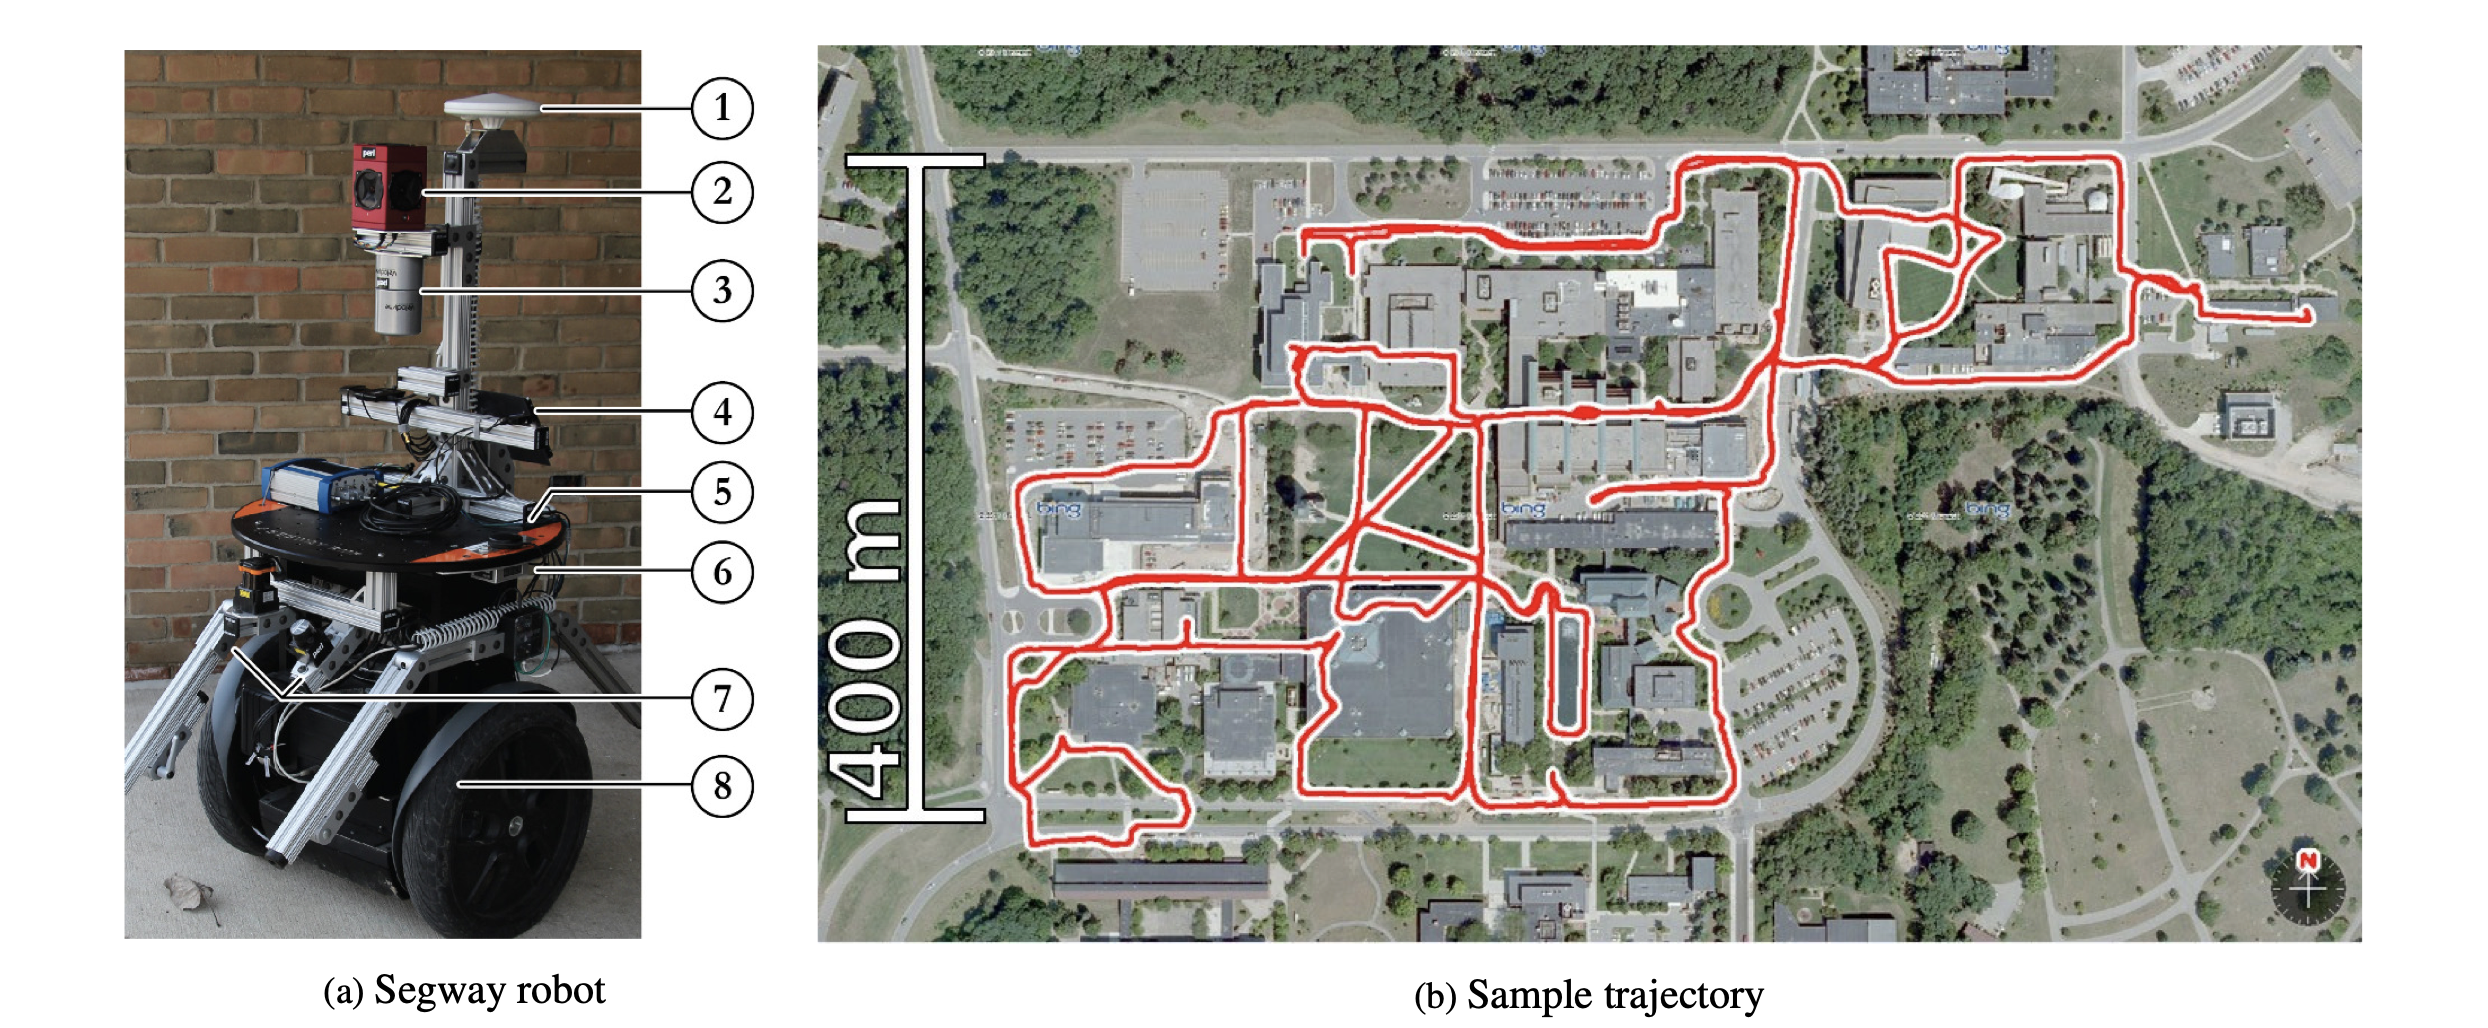
\includegraphics[width=1\columnwidth]{media/Robot_intro.png}
    \caption{The Segway robotic platform used for experimental data collection from NCLT.}
    \label{fig:Robot}
\end{figure}
